\documentclass[english,a4paper,12pt]{report}
\usepackage{babel}
%%\usepackage[latin1]{inputenc}
%%\usepackage{amsfonts}
%%\usepackage{stmaryrd}
%%\usepackage{amssymb}
%%\usepackage{latexsym}
%%\usepackage{cite}
\usepackage{graphicx}
%%\usepackage[small,bf]{caption}

\setlength{\textwidth}{18cm}
\setlength{\oddsidemargin}{-1.04cm}

\newcommand{\dftd}{\textsf{Danger from the Deep}}

\title{A guide to the sourcecode of \dftd}

\begin{document}

\titlepage

\tableofcontents

%define commands to format strings
% like \code{bla} for a specially formatted bla, like texttt

% talk about multithreading, explain what is planned and why its not yet done
% beginners: check carefully what you want to do, it may be already implemented
% beginners: philosophy different? do not start to change code wildly
% talk about the 3d format (ddxml)
% why c++? give examples, do not defend language too much, its a ``take it or leave''
%  e.g. memory management is different to Java AND different to C.
% make code style shorter, less excusing, just a ``do it that way''
% explain texture/image and the idea, basic classes like system
% maybe rename to ``Developer's guide to DftD''
% talk about data formats (xml), in savegames, specfiles and so on
% talk about documentation: doxygen, many, many things missing here.
% draw some uml diagrams for the important classes (subsection of full graph) and embed
%  them here as eps graphics.

\chapter{About this document}

What is this document about? It should give you a general overview of
the sourcecode of \dftd, the general concepts and ideas. Most projects
of today come with a code-related documentation (like Doxygen). This is
generally a handy thing, when developing or extending code - \dftd\ has
it too (many things are still missing). But it helps you only when you
know where to look and \emph{how} to extend the code.  Even if the code
would have a documentation for \emph{every} function, you would not know
where to start. Code-based documentation can be the final step to make
project documentation complete, but it is not useful as first step into
the project. It is often misused as excuse to not creating a more
general documentation.

Many open source projects out there have a more or less well managed
Doxygen-like code documentation. But what is it good for? It is of use
only for those that already know how to use the project - as reference.
But where to start if you are new to the project? You are lost. At that
point example code may help or researching for information on the
internet. Or to consult a more general documentation, if available.

For this project, only the latter option is possible (or you enter
IRC/forum and ask us directly, what you should do anyway if you want to
join). This document tries to solve the problem described above and
tries to give interested people an overview of the project.

Of course one could enhance the Doxygen-based documentation while
learning more about the project. Such a person would be very welcome.

\chapter{General idea}

This is a hobby project. All developers do the work in their spare time,
no one is paid for it. The code has grown for years (since around
january 2003) and many people contributed to it. While we worked on the
project, we changed many things: interfaces, implementations and
algorithms. We tried many things. While developing the code, our
knowledge developed as well. Thus, the style of writing code and using
C++ changed as well. As a result of all these facts, you will find out
that the code is not as uniform as code could be.

However, i can tell you from real life experience (working as software
engineer), that this is true for the most code on this planet.
Considered that fact, the source code of \dftd\ could be much worse. The
code is made after the object oriented paradigm about software
construction. Its extensible, mostly readable and understandable. Beside
aiming for functionality we aim for speed too, as we are working on a
game with realtime effects.  For that reason we use \emph{C++}, as it
features object orientation, high execution speed and flexibility as
well.

The game is written in portable code and can be compiled for many
platforms (up to six working at end of 2006). The text resources inside
are not hardcoded, so the game supports multiple languages (currently
seven are implemented at end of 2006). Now consider that we are working
on a realtime 3d game with many great visual effects, multi platform,
multi language and many more features.

\section{Joining}

If \emph{you} want to join the team, then you are welcome. We need more
developers. But let me tell you one warning word first. This is not
meant to offend you, but to make you think. Please read on.

People tend to transfer their view of coding to new projects, trying to
adapt the project to their style. You may be a smart and brilliant
coder, you may believe that your way of doing things is the best, no
matter what way the project has chosen before you joined. We don't want
to hinder you to start hacking on the code, extending it with more
features or fixing bugs et cetera.  Any help or contribution is
appreciated. But\ldots there comes the warning.

But\ldots the point is, if you do so, check carefully what you do and
how you do it. The feature you want do implement may have been already
implemented, somewhere more or less hidden in the code. The aspect you
want to add may collide with some other parts of the code. The functions
you add may conflict with existing interfaces. The way you want to
implement a feature, may be only one alternative of many, and possible
not the ideal one, and so on.

This is not meant to offend you, the contributor of new code. I write
this to avoid double work. To avoid wasting your time with writing code
that already exists or wasting time of others by breaking existing code.
If you want to contribute, I stronlgy recommend to get a copy of the
code and try to understand what is going on inside it first. One step of
that process is to read this document so you are on the right path.

\section{History}

The game arised from a graphic test for OpenGL under Linux. I wanted to
try out OpenGL graphics under Linux and finally wrote some tile based
water rendering code. Later i added a simple model loader and had the
very basics of a submarine simulation. As i am a great fan of Silent
Service and Aces of the Deep (guess where the name comes from) and
considered the fact that there is or was no submarine simulation for
Linux, i began to create one.
    
The project started in January 2003 and the code evolved since that
time. I improved my knowledge about C++, OpenGL and about software
development in general. Other developers joined the project and added
more ideas and development ideas and styles. Often things were just
tried out and thrown away later. This all lead to code that seems a bit
chaotic, more like evolution and less planned. There are many places
where this can be seen. Interfaces that are not fully implemented, or
various ways doing similar things around the code.
  


\section{Used libraries}

SDL, SDL\_image, fftw, SDL\_mixer, SDL\_net

\section{Language: C++}

speed, object orientation, platform independence, opengl, flexibility (multiple inheritance)

\subsection{About resource and memory management}

I bet you have been told that there are two models of handling resources
like files, memory and more: the \emph{C}-like way, where you have to do
everything on your own and the \emph{Java}-like way, where some entity
called ``garbage collector'' cleans up unused memory for you. The same
is true for other resources, except that even such an collector could
not know when to close files and you have to close them at the right
time like with \emph{C}.

The \emph{C}-way is problematic, because you have to do every tiny bit
of work for yourself and you have to do it over and over again, which is
highly error prone.

On the other hand there is the clean OOP-way (object oriented
programming), where memory doesn't need to be freed by the the
developer, but the runtime environment does it for you. Of course that
environment can't know when to close files, so you have to do this still
on your own. When code can throw exceptions, you have to encapsulate
file handling and close them in special code blocks (the \emph{final}
keyword in \emph{Java}) or similar things.

In fact, there is a third way. The only language i know that offers this
way is \emph{C++}. You can do it the hard way like \emph{C} but you
should not. \emph{C++} is not \emph{C}. The language follows a very
different paradigm. And \emph{C++} is not like \emph{Java}. There are
critical differences. Do the things in \emph{C++} like they should be
done in this language, and not like \emph{C} and not like \emph{Java}.
The \emph{C++} paradigm is not that hard to learn and brings you some
surprising advantages.

The key mechanism is that local variables can be objects. Local
variables are local to the block they are defined in (from opening curly
brace to closing curly brace). If the variable is an object of some
class, the constructor of that class is called on defining the variable,
and the destructor is called automatically when leaving the block.
Constructors and destructors are more or less normal functions, so you
can put any code in them. The object you declare does not even have to
have attributes with it, its constructor and destructor is called
anyway.

I hope you already see what enormous chances this offers. Automatic call
of a function when leaving a block? No matter how the block is left - by
either normal code execution or break or return or exception? This fits
perfectly to closing a file or freeing memory.

By letting \emph{C++} handle the local variables automatically and by
attaching resources to such local variables you can make nearly
\emph{every} resource management automatic! Never ever again you lose
some memory or forget to close files. Resources are automatically freed
when an error occurs and the code is stopped by an exception. Stable,
reliable design without extra work by the developer - doesn't that sound
great?

It \emph{is} great, but the price is language complexity and some extra
work on declaring such helper classes. But the first problem vanishs
once you are used to the language, and the second problem is tiny
compared to the advantages you can enjoy with the method.

The \emph{C++} standard library (STL) already makes use of such
techniques and has fully automatic memory management. Full speed of
\emph{C} with the easy coding like \emph{Java} (sometimes even easier).
That is one of the reasons why we have chosen to use \emph{C++} for the
project.

The automatisms can be seen in the standard classes like
\texttt{std::vector} or \texttt{std::auto\_ptr}, and are also used by
some \dftd\ classes like the \texttt{ptrset} or the \texttt{ptrvector}.
The concept is used for files too, realized as ``streams'' in
\emph{C++}. It can be extended very well to multi-threaded programming
as well, like writing a class that locks a mutex in constructor and
unlocks it in its destructor. That way mutex locking can be done
automatically by declaring such a locker object inside a code block.
Upon leaving the block, the mutex is automatically unlocked, removing a
very nasty and common source of error with multi-threaded programming.
Many more applications are possible.

In short one can say: if you use \texttt{new} and \texttt{delete} to
allocate memory blocks, you do something wrong. Use vectors instead. You
should only create single objects with new and should attach them
directly to an object that can manage the memory automatically, so the
object can not get lost, whatever happens (exceptions can break normal
code flow, be careful!). Thus, you should not be forced to use
\texttt{delete} too often. If you even would use \texttt{malloc} or
\texttt{free} anywhere, you are very wrong and should expect harsh
comments by the developers. These functions are exclusivly \emph{C} and
do not mix with the \emph{C++} ones. As the \emph{C++}-FAQ ``lite'' by
Marshall Cline abbreviates it: arrays are \emph{evil}, unmanaged
pointers are \emph{evil} - in general. Check if you could use a
\emph{reference} instead of a pointer, whereever you would like to use
pointers.

I suggest reading the mentioned FAQ at
http://www.parashift.com/c++-faq-lite/

\section{Error handling}

Currently the code treats errors as fatal events, reports it via message
to command line and quits the game. Checks are done using the
\textbf{system::myassert()} function, but this is embarassing and ugly.
This mixes code test related assertions with error checks.  C++
exceptions are the definite thing to use here, but are used very rarely
yet. I discovered only recently how useful they are.
    
The whole code (that means each place with a \textbf{system::myassert()
  call} has to be checked wether it is an error check (in that case
replaced by an descriptive exception) or a development check (in that
case a normal \textbf{assert()} could be used). For exceptions one
should define classes that heir from \textbf{std::exception} and contain
an error string. A hierarchy of exceptions could be created for a finer
grained error handling and control. Look at file \textbf{error.h} for an
example definition.

The general idea about exceptions is to report \emph{what} went wrong,
not where. Exceptions are made to handle errors at runtime. If you want
to know where the error was raised to ease development, add a
descriptive text to the exception or print it in the log. Each exception
can be given a report text that is for the user or developer. With some
tricky macros you can append the line and source file name to the text
as well (see file \texttt{error.h}). The set of exceptions brought by
the C++ standard library is a good starting point and these exceptions
already cover many possible errors, like \texttt{invalid\_argument},
\texttt{runtime\_error} and so on. The constructor of an exceptions gets
an user defined string, where a developer can state the nature of the
error.

For example you could check in some function, if a given pointer is
non-zero:
\begin{verbatim}
if (!myptr)
        throw std::invalid_argument("myfunction: Null-pointer given");
\end{verbatim}
(Of course if you expect some pointer to have a valid value, you maybe
could use a reference instead).

All exceptions form an inheritance tree, a hierachy. Because of that one
can categorize errors and handle them regarding to category. This allows
a very flexible error management. I suggest you to learn something more
about C++ exceptions if you are new to the language. The C-style of
error reporting via return values is \emph{not} the way to do it. But do
not confuse error handling by value reporting. If a function should do a
simple thing that can fail, it would be ok to return a bool for that
function and not throw an exception in case of error. It depends on the
severity and if the caller can handle that malfunction directly.

Good examples where to use exceptions are situations where errors are
not expected, where normal code execution is assumed. As their name
already tells, exceptions are designed to handle exceptional situations.
You want to load an image and can't read the file? Then throw an
exception. The exception will be e.g. passed upwards to the mission
loader, which can react on it. For example it could present an error
message to the user: ``couldn't load mission, because of \ldots'' or
similar things.

Final note: because exceptions break normal control flow of programs,
you have to write your code in a way that no memory is lost or resource
is kept. If you do a thing that needs to be cleaned up when leaving the
current block of code, you need to embrace the code with a try/catch
clause and clean up in the catch-path. You can make your life much
easier, if you use built-in types that do this automatically. For
example use auto-pointers (\texttt{std::auto\_ptr}) instead of plain
C-pointers or streams (\texttt{std::ifstream}) instead of file-pointers.
A very handy thing is to add a class that does the cleanup in its
destructor (and the initialization in the constructor) and to
instantiate an object of that class as local variable. The compiler then
will automagically do all the clean-up work for you.


\chapter{Structure of the project}

Class diagram:

\begin{figure}[ht]
\centering
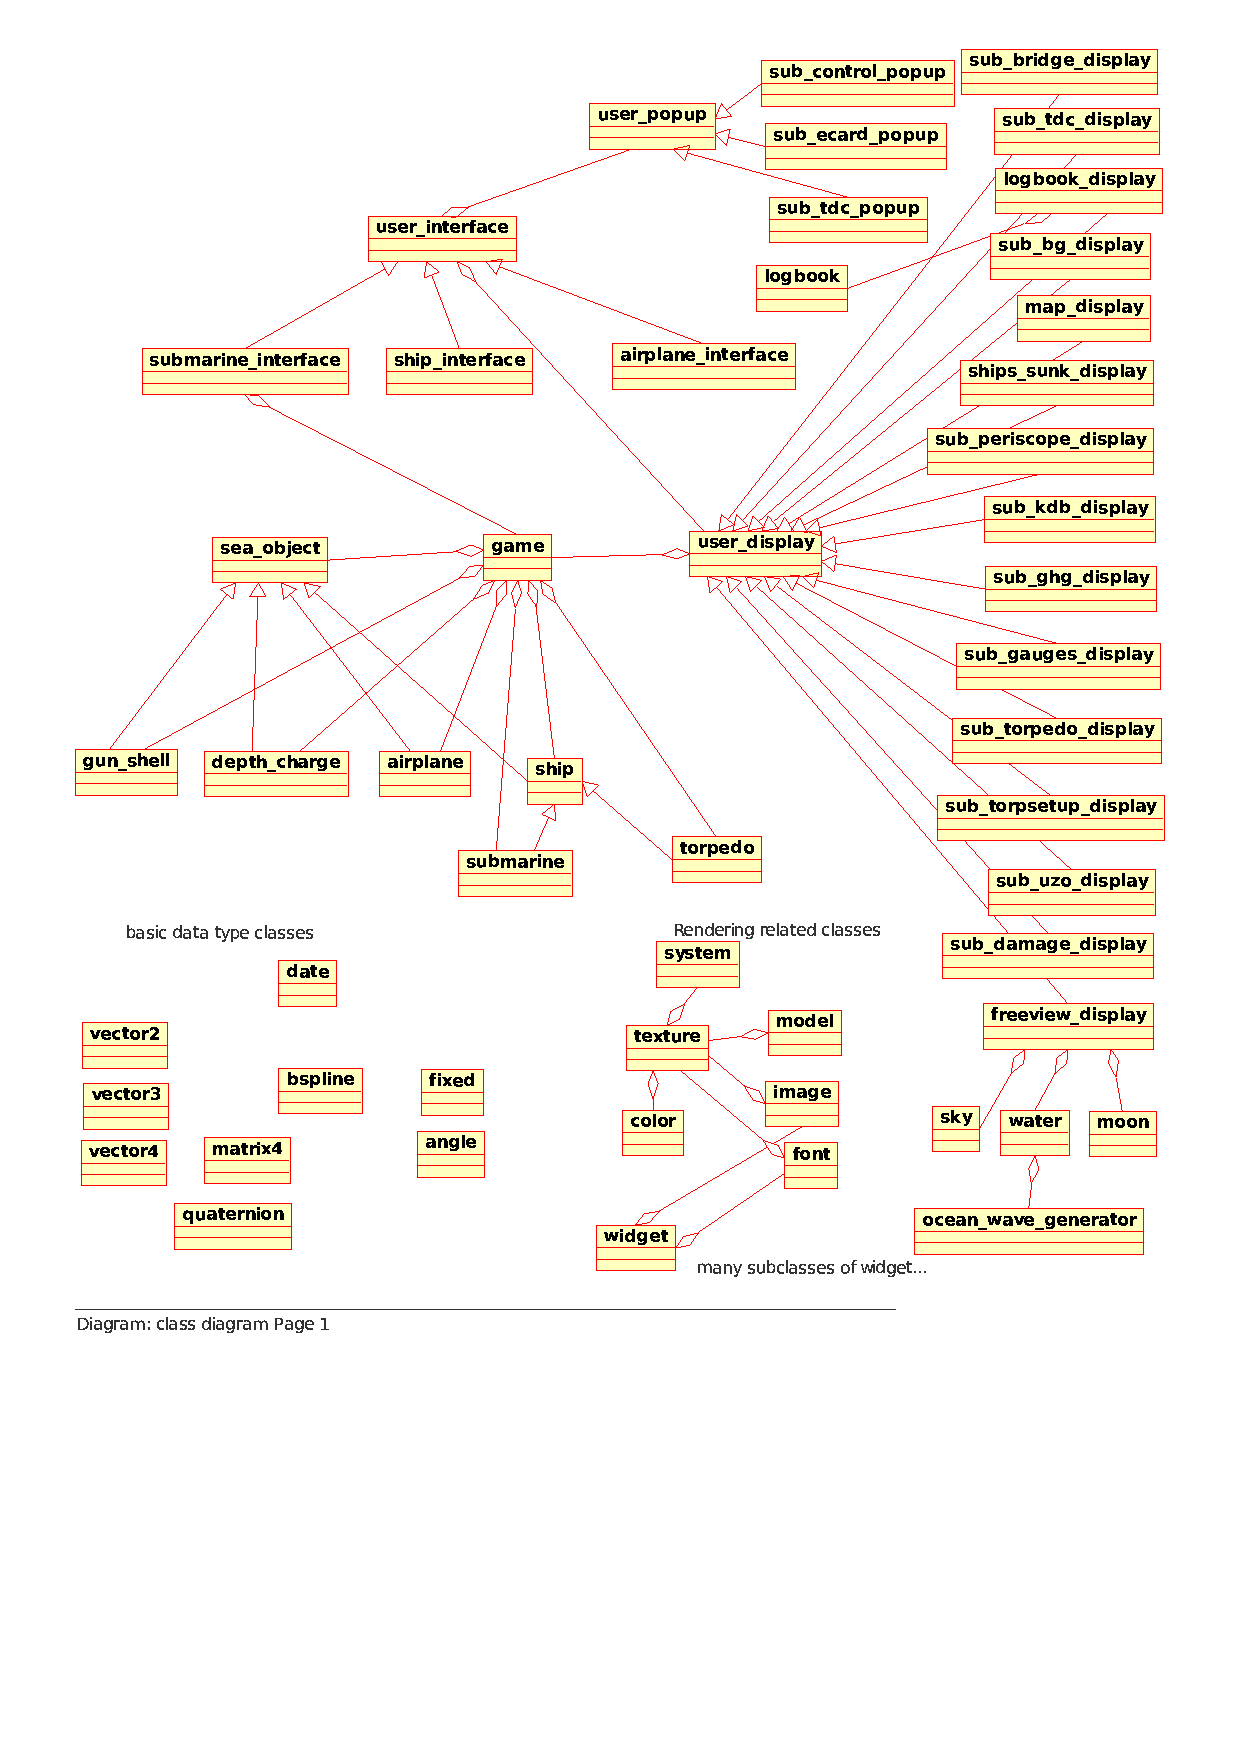
\includegraphics[width=18cm]{classdiagram}
\caption{Class diagram of \dftd}
\label{classdiagram}
\end{figure}

\section{Main files and interfaces}

At the writing of this document the games has several dozen header and
source files (classes). It takes some work to learn which file does what
and how. As a short guide I explain the main files and interfaces here.

\subsection{Where it all starts}

Check the file \texttt{subsim.cpp}. This file contains the \texttt{main}
function of the game. There game objects are created, user interfaces
are initialized and so on. You need to learn about the other interfaces
first to understand that file.

\subsection{State and display}

The central aspect is playing a game. The code is divided in two
categories. One for handling the state of the game, that is storing all
objects, their data, simulating physics, environment and so on. The
other part is the presentation of that data: visualization, sound
processing, user input.

\subsection{Hierachy of state classes}

The central class for a game instance is the class \texttt{game}. That
class describes an instance of a game at any time and holds all other
objects needed to represent a game's state. The class \texttt{game}
holds all objects of the game's world like airplaines, ships,
submarines, grenades, torpedoes and so on. Every object in the game that
is a physical entity is of class \texttt{sea\_object} or one of its
heirs.

Heirs of \texttt{sea\_object} are e.g. \texttt{ship}, \texttt{airplane},
\texttt{gun\_shell} and so on. Heirs of \texttt{ship} are e.g.
\texttt{submarine} and \texttt{torpedo}. Now you see what we need
multiple inheritance for.

The game object and all incorporated objects are the data representation
of the simulated word. Their contents are stored in savegames. If you do
something about simulating the world or its content, you modify any
object attached to the game object.

\subsection{Hierarchy of presentation classes}

On the other side, there are the classes used for user input and
graphical output (well, sound and music as well). I describe the user
interface here, that is merely the graphical interface.

The central class of the user interface is called so:
\texttt{user\_interface}. Everything needed to render the game or
environment is attached to it. There are implementations depending on
the type of object that the player controls:
\texttt{airplane\_interface}, \texttt{ship\_interface} and
\texttt{submarine\_interface}, where at the moment only the latter is
funtional. The interface object also holds classes for displaying the
sky, sun, moon, the ocean environment and the environment of the player
controlled vessel.

The in-game user interface is partitioned in multiple screens or
displays, also known as stations. For example the various compartments
of a ship or submarine: the bridge, the engine room, the map chart et
cetera. The base class for such a screen is \texttt{user\_display}.
Every display heirs from it, and there are many.

% interface is only display or input<->output, so game is const while display

% popups

\section{Basic classes and types}

\subsection{Mathematical helper classes}

There are some basic classes that implement various mathematical
constructs as template classes, so one can instantiate them for any
needed data type. Predefined names for \texttt{int}, \texttt{float} and
\texttt{double} exist. These base classes are for vectors
(\texttt{vector2}, \texttt{vector3} and \texttt{vector4}), matrices
(\texttt{matrix4}) and quaternions (\texttt{quaternion}). Operator
overloading is used so that one can write equations and formulas in a
common style. The code is rather self explanatory, so have a look.

There is also a helper class for (nautical) angles: \texttt{angle}, that
implements wrapping of values at 360 degrees and some other useful
things.

And finally a helper class for fixed point arithmetic data types:
\texttt{fixed}. Fixed point arithmetic is still faster for some cases
and the precision is still high enough for some tasks related to 3D
rendering (do not use them for physics though, nor \texttt{float}, but
\texttt{double} for physics).

\subsection{Other helper classes}
    
bspline color data error filehelper fixed objcache ptrset

\subsection{Rendering and system related related classes}

model.h sound.h texture.h font.h network.h color.h image.h system.h

\subsection{Components of the game state and simulation}

ai.h airplane.h game.h torpedo.h submarine.h gun_shell.h convoy.h
sea_object.h sensors.h ship.h depth_charge.h

\subsection{Components of the graphical user interface}

sub_bridge_display.h airplane_interface.h freeview_display.h
sub_control_popup.h sub_damage_display.h sub_gauges_display.h
submarine_interface.h user_display.h sub_periscope_display.h
user_interface.h sub_tdc_display.h user_popup.h sub_tdc_popup.h
logbook_display.h sub_torpedo_display.h logbook.h
sub_torpsetup_display.h ship_interface.h sub_uzo_display.h map_display.h
ships_sunk_display.h

\subsection{Special 3D rendering related classes}

ocean_wave_generator.h particle.h triangulate.h perlinnoise.h coastmap.h
sky.h water.h water_sse.h make_mesh.h

\subsection{OpenGL GUI classes}

widget.h

\subsection{Miscellaneous classes}

tokencodes.h token.h tokenizer.h binstream.h gldebug.h parser.h
global_data.h cfg.h highscorelist.h keys.h texts.h credits.h




\section{The game: state and display, the classes \texttt{game} and
  \texttt{user\_interface}}

The code (functionality, data structures and classes) of the game is
partitioned in two parts: one managing the state and the other managing
the display or user interface. The central class for the state data is
the class \texttt{game} with all its dependant classes
(\texttt{sea\_object} and its heirs and so on). All data you need to
describe a game's state is stored there. If you want to save games or do
network play, all data you have to access is hold by that class.

On the other side there is the user interface. Its heirs and associated
classes manage everything from state presentation (visual and acustical
- graphic and sound) to user interaction (input). This part requests
data from the \texttt{game} class for presentation. Parts of the user
interface for example are the classes for the stations, the
environmental rendering (classes \texttt{water}, \texttt{sky},
\texttt{moon}, \texttt{user\_display} and many more).

To simulate the game one only needs to change the class \texttt{game}
and its corelated data. This class knows nothing about the user
interface. Because of that you can use one instance of the
\texttt{user\_interface} class with any instance of class \texttt{game}
without the need to reconstruct the user interface, which is a costly
process. You can instead simply exchange the game object, as it is done
for loading games or as it would be needed for network play or switching
missions.

Note that at the moment there is a reference to \texttt{user\_interface}
in class \texttt{game}, that is needed for simulation. The main loop of
the game is currently in \texttt{game::run()}, which needs to know the
user interface instance. However it is planned to resolve that situation
and move the main loop code outside of class \texttt{game}. Then we have
the real partition between two parts, as described above. However if you
plan to add features, always keep this partition in mind.

And why do we do that? Doesn't it make thing more complicated? No, it
isn't a real limitation, but on the other hand splits code in two clean
domains. Physical simulation and rendering are two independent parts. It
would be a lot more complex if state simulation would interact with the
user interface in every possible situation.

Note that events causing feedback to the user (like playing an explosion
sound after a collision) need some extra work. You can't simply call an
``play explosion'' function of the user interface (where the sound is
played) from class \texttt{game} (where you detect the collision).
Instead you have to remember such events in class game and let the user
interface request the events and react on them.

This partitioning brings problems as you see, but also has its
advantages. You can simulate the game without need to render it. This
allows dedicated servers. Or it allows to exchange the renderer or many
more things.


\chapter{Coding style}

\section{Introduction}
This is a topic that can cause more heat than light when discussed.
Everyone has and likes his own style. Anyway, this here is the style we
use in the source code of \dftd. You have been warned.

It is desireable to use \emph{one} style throughout the whole code to
enhance readability. But creating working code is of course more
important than keeping style consistent at any cost. If you create new
code and have the choice, you should use the game's style to enhance
readability though.  Code that was contributed by other people may have
a different style, this is the case in some parts of current code.

This style originated from the ideas of the coding style of the Linux
Kernel (originally written by Linus Torvalds). Although everyone likes
his own style and mostly there are arguments pro or contra a certain
style, this one is reasonable. See below.
    

\section{Indentation}
People differ on how many spaces to indent. In my opinion everything
less than four is a pain. I use eight, because this will really help one
to see \textbf{how} indentation works (and even after sitting many hours
in front of the monitor). The simple solution to this problem is: use
\textbf{TABs} for indentation. Everyone can set his favorite tab width
in his editor then. There is another reason: indenting that much
prevents you from nesting your code to deep, which is a good help to
avoid too complex code.
    

\section{Placing (curly) braces}

Yes, the old C discussion. I place braces at the end of the line of the
command. Want an example? here it comes:
    
Conditional commands:
    
\begin{verbatim}
if (x == 3) {
        do_something();
} else if (y == 4) {
        do_other();
} else {
        do_another();
}

switch (a) {
case 3:
        do_abc();
        break;
case 4:
        do_efg();
}
\end{verbatim}

    Various loops:
    
    \begin{verbatim}
for (unsigned i = 0; i < 3; ++i) {
        b += z;
}

do {
    do_nothing();
} while (z == 5);

while (true) {
        do_something();
}
\end{verbatim}

    Functions and classes:
    
    \begin{verbatim}
void foo(int i)
{
        do_func_code();
}

class xyz : public abc
{
 private:
        int a;
 public:
        xyz();
};
\end{verbatim}

    Why this style? Kernighan and Ritchie used it and when XEmacs is set
    to this style it produces this kind of style and its auto-formatting
    works best with it. Seriously, this style leads to code that wastes
    less space (especially saves lines!) without losing readability.
    I've seen much code that places each brace in its own line at the
    cost that the code is much longer. The longer it gets, the less fits
    on one screen and one needs to scroll, which makes it more difficult
    to follow the execution path of the code and to understand it.
    

    \section{Naming}

    I prefer using lowerspace characters and underscores. Why? humans
    are more trained to read lowerspace characters and underscores are a
    better optical partition than mixing lowerspace and upperspace
    characters. Example: read this fast and see what is easier.
    Lowerspace \textbf{this\_variable\_has\_a\_very\_long\_name}.
    Upperspace \textbf{thisVariableHasAVeryLongName}. Horrible. Looks
    crowded to me. If you write code for \dftd, please follow the rules
    and use underscores and not mixed-case names.
    
    The same goes for classes, members and functions. All should be in
    lowerspace form. Methods that return some data from a class should
    be named \textbf{get\_xyz()} when \textbf{xyz} is the name of the
    member. This is no hard rule, but it should be followed for
    consistency.
    
    The most important thing, and the only rule i urge you to really
    follow is to \textbf{not use hungarian notation} nor anything
    similar. This is a very weird thing some big, greedy software
    company introduced and makes code \textbf{hard to read}. The
    compiler will check the type of the variables anyway, and if you
    state that you would need this kind of notation to show what your
    variables are or do, you did something wrong before. If you can't
    tell from the name of a variable what it does, then this is the real
    problem. Adding the type to the name doesn't fix it.

    Cause of the real problem: maybe you also have too many variables so
    that you want to add the type to distinguish between them? Another
    problem is the reason: don't make functions or classes too long or
    too complicated!
    

    \section{Closing words}

      These rules are no strict "you must follow them" rules. I prefer
      working code is added to the game rather than keeping the style
      conform. But it can help to read and understand the code, so
      please try to keep the style.
    
    \chapter{What needs to be done}

    \section{Janitors wanted}


 \end{document}
